\documentclass[11pt]{article}

% ---------------------------------------------------------------------------
% Packages
% ---------------------------------------------------------------------------
\usepackage[margin=1in]{geometry}
\usepackage{amsmath, amssymb, amsthm, bm}
\usepackage{booktabs, tabularx, array}
\usepackage{graphicx}
\usepackage{float}
\usepackage{enumitem}
\usepackage{xcolor}
\usepackage[colorlinks=true, linkcolor=blue, urlcolor=blue, citecolor=blue]{hyperref}

% Overleaf: upload the PNGs from the repo's figures/ folder into a folder named figures/
\graphicspath{{figures/}{../../figures/}}

% ---------------------------------------------------------------------------
% Theorem environments
% ---------------------------------------------------------------------------
\theoremstyle{definition}
\newtheorem{definition}{Definition}[section]
\newtheorem{assumption}{Assumption}
\theoremstyle{plain}
\newtheorem{theorem}{Theorem}[section]
\newtheorem{proposition}[theorem]{Proposition}
\newtheorem{lemma}[theorem]{Lemma}

% ---------------------------------------------------------------------------
% Macros
% ---------------------------------------------------------------------------
\newcommand{\R}{\mathbb{R}}
\newcommand{\E}{\mathbb{E}}
\newcommand{\Var}{\operatorname{Var}}
\newcommand{\Cov}{\operatorname{Cov}}
\newcommand{\tr}{\operatorname{tr}}
\newcommand{\x}{\mathbf{x}}
\newcommand{\z}{\mathbf{z}}
\newcommand{\bmu}{\bm{\mu}}
\newcommand{\hmu}{\hat{\bm{\mu}}}
\newcommand{\hSigma}{\hat{\Sigma}}
\newcommand{\one}{\mathbf{1}}
\newcommand{\Normal}{\mathcal{N}}

% Mark each step of a proof with the rule used:  \rulenote{linearity of expectation}
\newcommand{\rulenote}[1]{\quad\text{\small\color{gray}[#1]}}
% Owner / checker line under every derivation
\newcommand{\signoff}[2]{\par\smallskip\noindent\textit{Owner: #1 \quad\textbar\quad Checked by: #2}\par\medskip}
% Placeholder text
\newcommand{\todo}[1]{\textcolor{red}{\textbf{TODO:} #1}}

% ---------------------------------------------------------------------------
\title{DS5020 Final Project -- Iteration 2\\[4pt]
\large Anomaly Detection with the Multivariate Normal Distribution\\
The Math Foundation: Definitions, Derivations, Data and Simulations}
\author{Bijun Wu \and Kanchan Patkar}
\date{\today}

\begin{document}
\maketitle

\noindent\textbf{GitHub:} \url{https://github.com/WUB8/ds5020-anomaly-detection}\\
\textbf{Project Leader (Iteration 2):} \todo{name}

% ===========================================================================
\section{Task Table}
% ===========================================================================
\begin{table}[H]
\centering
\begin{tabular}{@{}llllc@{}}
\toprule
ID & Task & Owner & Checker & Status \\
\midrule
T1 & Notation and definitions                 & Bijun   & Kanchan & Done \\
T2 & Assumptions                              & Kanchan & Bijun   & Done \\
Q1 & MLE of $\bmu$ and $\Sigma$               & Bijun   & Kanchan & \todo{} \\
Q2 & Mahalanobis distance is non-negative     & Bijun   & Kanchan & \todo{} \\
Q3 & $d^2 \sim \chi^2_d$                      & Kanchan & Bijun   & \todo{} \\
Q4 & $\Sigma^{-1/2}$ from eigendecomposition  & Kanchan & Bijun   & \todo{} \\
Q5 & False-alarm rate equals $\alpha$         & Kanchan & Bijun   & \todo{} \\
T3 & Algorithm as math                        & \todo{} & \todo{} & \todo{} \\
T4 & Real data description                    & Bijun   & Kanchan & Done    \\
T5 & Simulation check                         & Bijun   & Kanchan & Done    \\
\bottomrule
\end{tabular}
\end{table}

% ===========================================================================
\section{Notation and Definitions}
% ===========================================================================
\subsection{Notation}
\begin{table}[H]
\centering
\begin{tabularx}{\textwidth}{@{}l l X@{}}
\toprule
Symbol & Dimension & Meaning \\
\midrule
$s$ & index & subject (typist), $s = 1,\dots,51$ \\
$u$ & index & the genuine user whose typing rhythm is modelled \\
$k$ & index & key of the password \texttt{.tie5Roanl} + Return, $k = 1,\dots,11$ \\
$H_k$ & scalar (s) & hold time of key $k$ (key-down to key-up) \\
$DD_{k,k+1}$ & scalar (s) & keydown--keydown latency between consecutive keys \\
$UD_{k,k+1}$ & scalar (s) & keyup--keydown latency; $UD_{k,k+1} = DD_{k,k+1} - H_k$ \\
$\x^{\text{raw}}_i$ & $\R^{21}$ & raw timings of typing $i$: $(H_1,\dots,H_{11},DD_{1,2},\dots,DD_{10,11})$ \\
$\x_i$ & $\R^{d}$ & feature vector of typing $i$, $\x_i = \log\x^{\text{raw}}_i$ (entrywise) \\
$n$ & scalar & number of training typings of user $u$ ($n = 200$) \\
$d$ & scalar & number of features ($d = 21$: 11 hold times + 10 DD latencies) \\
$X$ & $\R^{n\times d}$ & training data matrix of user $u$; row $i$ is $\x_i^\top$ \\
$m_{\text{gen}},\ m_{\text{imp}}$ & scalars & number of genuine ($200$) and impostor ($250$) test typings \\
$\one$ & $\R^{n}$ & vector of ones \\
$\bmu$ & $\R^{d}$ & true mean vector \\
$\Sigma$ & $\R^{d\times d}$ & true covariance matrix (symmetric positive definite) \\
$\hmu,\ \hSigma$ & $\R^{d},\ \R^{d\times d}$ & maximum-likelihood estimates of $\bmu,\Sigma$ \\
$X_c$ & $\R^{n\times d}$ & centred data matrix, $X_c = X - \one\hmu^\top$ \\
$Q$ & $\R^{d\times d}$ & orthogonal matrix of eigenvectors of $\Sigma$ \\
$\Lambda$ & $\R^{d\times d}$ & diagonal matrix of eigenvalues $\lambda_1,\dots,\lambda_d$ of $\Sigma$ \\
$\Sigma^{-1/2}$ & $\R^{d\times d}$ & inverse square root, $Q\Lambda^{-1/2}Q^\top$ \\
$\z$ & $\R^{d}$ & whitened vector, $\z = \Sigma^{-1/2}(\x - \bmu)$ \\
$d^2(\x)$ & scalar & squared Mahalanobis distance of $\x$ \\
$\ell(\bmu,\Sigma)$ & scalar & log-likelihood \\
$\alpha$ & scalar & target false-alarm rate \\
$\tau$ & scalar & threshold, $\tau = \chi^2_{d,1-\alpha}$ \\
\bottomrule
\end{tabularx}
\end{table}

\subsection{Connecting the Data to the Math}
\paragraph{Dataset.} CMU Keystroke Dynamics Benchmark (Killourhy and Maxion, 2009). Each of 51 subjects typed the password \texttt{.tie5Roanl} followed by Return 400 times: 8 sessions of 50 repetitions, with sessions on different days. The file has $51\times400 = 20{,}400$ rows. Each row contains \texttt{subject}, \texttt{sessionIndex}, \texttt{rep} and 31 timing features in seconds: 11 hold times $H_k$, 10 keydown--keydown latencies $DD_{k,k+1}$ and 10 keyup--keydown latencies $UD_{k,k+1}$.

\paragraph{One row, one column, one entry.}
\begin{itemize}[leftmargin=*]
\item \textbf{One row} $\x_i^\top$ of $X$ is one complete typing of the password by user $u$.
\item \textbf{One column} $j$ of $X$ is one timing feature across all typings, e.g.\ the hold time of the key \texttt{t}, or the keydown--keydown latency from \texttt{t} to \texttt{i}.
\item \textbf{One entry} $X_{ij}$ is the log of that timing, in log-seconds, for typing $i$.
\end{itemize}

\paragraph{Feature choice.} We use $d = 21$ features: the 11 hold times and the 10 $DD$ latencies. The 10 $UD$ latencies are dropped because they are an exact linear combination of the others, $UD_{k,k+1} = DD_{k,k+1} - H_k$. Keeping all 31 would make $\Sigma$ singular (Assumption~\ref{as:pd}). Using $DD$ rather than $UD$ also keeps every feature positive, so the log transform is defined ($UD$ can be negative when two keys overlap).

\paragraph{Normal vs.\ anomalous.} For each genuine user $u$ we follow the benchmark's protocol: the first $n = 200$ typings (sessions 1--4) are the training data used to fit $\hmu,\hSigma$. The test set is the remaining $m_{\text{gen}} = 200$ typings of $u$ (normal), plus the first 5 typings of each of the other 50 subjects, $m_{\text{imp}} = 250$ (anomalies, i.e.\ impostors). We repeat this with every subject as the genuine user.

\subsection{Definitions}
\begin{definition}[Symmetric positive (semi-)definite matrix]
$A\in\R^{d\times d}$ is symmetric if $A^\top = A$. It is positive semi-definite if $\mathbf{v}^\top A\mathbf{v}\ge 0$ for all $\mathbf{v}\in\R^d$, and positive definite if $\mathbf{v}^\top A\mathbf{v}>0$ for all $\mathbf{v}\neq\mathbf{0}$.
\end{definition}

\begin{definition}[Mean vector and covariance matrix]
For a random vector $\x\in\R^d$, the mean vector is $\bmu = \E[\x]\in\R^d$ and the covariance matrix is
\[
\Sigma = \E\big[(\x-\bmu)(\x-\bmu)^\top\big]\in\R^{d\times d},
\qquad
\Sigma_{jk} = \Cov(x_j,x_k) = \E\big[(x_j-\mu_j)(x_k-\mu_k)\big].
\]
The diagonal entries $\Sigma_{jj} = \Var(x_j)$ are the variances of the individual features.
\end{definition}

\begin{definition}[Multivariate normal distribution]
A random vector $\x\in\R^d$ has the multivariate normal distribution $\x\sim\Normal(\bmu,\Sigma)$, with $\Sigma$ symmetric positive definite, if its density is
\[
f(\x\mid\bmu,\Sigma) = \frac{1}{(2\pi)^{d/2}\,|\Sigma|^{1/2}}
\exp\!\Big(-\tfrac12(\x-\bmu)^\top\Sigma^{-1}(\x-\bmu)\Big),
\qquad \x\in\R^d,
\]
where $|\Sigma|$ is the determinant of $\Sigma$.
\end{definition}

\begin{definition}[Likelihood and maximum-likelihood estimator]
Given observations $\x_1,\dots,\x_n$ with joint density $f(\x_1,\dots,\x_n\mid\theta)$, the likelihood is the function $L(\theta) = f(\x_1,\dots,\x_n\mid\theta)$ of the parameter $\theta$ with the data held fixed, and the log-likelihood is $\ell(\theta) = \log L(\theta)$. The maximum-likelihood estimator (MLE) is
\[
\hat\theta = \arg\max_{\theta}\, L(\theta) = \arg\max_{\theta}\, \ell(\theta).
\]
Here $\theta = (\bmu,\Sigma)$.
\end{definition}

\begin{definition}[Eigenvalue, eigenvector, spectral decomposition]
A scalar $\lambda$ is an eigenvalue of $A\in\R^{d\times d}$ with eigenvector $\mathbf{q}\neq\mathbf{0}$ if $A\mathbf{q} = \lambda\mathbf{q}$. By the spectral theorem, every real symmetric matrix $\Sigma$ can be written
\[
\Sigma = Q\Lambda Q^\top,\qquad Q^\top Q = QQ^\top = I,\qquad \Lambda = \operatorname{diag}(\lambda_1,\dots,\lambda_d),
\]
where the columns $\mathbf{q}_1,\dots,\mathbf{q}_d$ of $Q$ are orthonormal eigenvectors and $\lambda_1,\dots,\lambda_d$ are the corresponding real eigenvalues.
\end{definition}

\begin{definition}[Mahalanobis distance]
For $\x\in\R^d$, a mean $\bmu\in\R^d$ and a symmetric positive definite $\Sigma$, the Mahalanobis distance of $\x$ from $\bmu$ is
\[
d(\x) = \sqrt{(\x-\bmu)^\top\Sigma^{-1}(\x-\bmu)},
\]
and $d^2(\x) = (\x-\bmu)^\top\Sigma^{-1}(\x-\bmu)$ is the squared Mahalanobis distance. When $\Sigma = I$ it reduces to the Euclidean distance $\|\x-\bmu\|$.
\end{definition}

\begin{definition}[Chi-squared distribution]
If $Z_1,\dots,Z_d$ are independent $\Normal(0,1)$ random variables, then
\[
\sum_{j=1}^d Z_j^2 \sim \chi^2_d,
\]
the chi-squared distribution with $d$ degrees of freedom. It has mean $d$ and variance $2d$.
\end{definition}

\begin{definition}[Quantile and false-alarm rate]
For a continuous random variable $Y$ with cumulative distribution function $F$, the $(1-\alpha)$ quantile is the value $q_{1-\alpha}$ with $F(q_{1-\alpha}) = \Pr(Y\le q_{1-\alpha}) = 1-\alpha$. We write $\chi^2_{d,1-\alpha}$ for the $(1-\alpha)$ quantile of $\chi^2_d$. For a detector that flags $\x$ when $d^2(\x) > \tau$, the false-alarm rate is the probability that a normal reading is flagged,
\[
\Pr\big(d^2(\x) > \tau \;\big|\; \x\sim\Normal(\bmu,\Sigma)\big).
\]
\end{definition}

% ===========================================================================
\section{Assumptions}
% ===========================================================================
For each assumption: what goes wrong in the math if it fails, and how we will check it on the real data in Iteration 3.

\begin{assumption}[Independence and identical distribution]\label{as:iid}
The training typings $\x_1,\dots,\x_n$ of user $u$ are independent and all drawn from the same $\Normal(\bmu,\Sigma)$.\\
\emph{If it fails:} The likelihood in Q1 no longer factors into a product of densities, so $\hmu,\hSigma$ are no longer the exact MLEs. For keystrokes the main risk is \emph{practice and drift}: users get faster within a session and across the 8 sessions (different days), so the mean $\bmu$ changes over time. Consecutive repetitions within a session may also be correlated (fatigue, rhythm). A model trained on sessions 1--4 then sits away from the user's later typing in sessions 5--8, which inflates $d^2$ for genuine test typings and raises the false-alarm rate above $\alpha$.\\
\emph{Check:} Plot each feature (and the total typing time) against the repetition index $1,\dots,400$, coloured by session, and look for trends. Plot the autocorrelation of each feature within a session. Compare $\hmu$ fitted on sessions 1--2 with sessions 3--4.
\end{assumption}

\begin{assumption}[Normality]\label{as:normal}
For a fixed user, the log-timings follow $\Normal(\bmu,\Sigma)$.\\
\emph{If it fails:} Q3 ($d^2\sim\chi^2_d$) no longer holds, so the threshold $\tau = \chi^2_{d,1-\alpha}$ from Q5 does not give false-alarm rate $\alpha$. Raw timings are positive and right-skewed, with occasional very long pauses (heavy tails); our $t_3$ simulation shows heavy tails can make the false-alarm rate five times larger than $\alpha$. This is why we model $\log$ timings rather than raw seconds.\\
\emph{Check:} Histograms and normal Q-Q plots of each feature before and after the log transform. A Q-Q plot of the genuine users' $d^2$ against $\chi^2_{21}$. Compare the observed false-alarm rate on genuine test typings with $\alpha$.
\end{assumption}

\begin{assumption}[Positive definite covariance]\label{as:pd}
$\Sigma$ and $\hSigma$ are positive definite. This requires $n > d$ and that no feature is a linear combination of the others.\\
\emph{If it fails:} $\Sigma^{-1}$ and $\Sigma^{-1/2}$ do not exist, so $d^2(\x)$ is undefined (Q2, Q4). The dataset contains an exact linear dependence, $UD_{k,k+1} = DD_{k,k+1} - H_k$, so using all 31 raw features gives a singular $\hSigma$ with 10 zero eigenvalues. Even with $d=21$, strongly correlated features give tiny eigenvalues, and dividing by $\sqrt{\lambda_j}$ amplifies noise along those directions.\\
\emph{Check:} Confirm numerically that $UD = DD - H$ in the raw data. For each user, compute the eigenvalues of $\hSigma$ and the condition number $\lambda_{\max}/\lambda_{\min}$. If it is very large, add a small ridge $\hSigma + \varepsilon I$ and report its effect.
\end{assumption}

\begin{assumption}[Clean training data]\label{as:clean}
The 200 training typings are all genuine, typical typings of user $u$.\\
\emph{If it fails:} Unusual training typings (distractions, long hesitations) pull $\hmu$ towards them and inflate $\hSigma$. A larger $\hSigma$ means a smaller $\hSigma^{-1}$, which shrinks every $d^2$, so impostors look less unusual and are missed (masking).\\
\emph{Check:} Fit on the training set, list the training typings with the largest $d^2$, refit without them, and compare $\hmu,\hSigma$ and the detection results. The benchmark only contains correctly typed passwords, so typos are not a concern.
\end{assumption}

\begin{assumption}[Large sample]\label{as:large}
$n \gg d$, so that $\hmu\approx\bmu$ and $\hSigma\approx\Sigma$.\\
\emph{If it fails:} Q3 is exact only for the true $\bmu,\Sigma$; with plug-in estimates the distribution of $d^2$ is only approximately $\chi^2_d$, and the false-alarm rate drifts away from $\alpha$. Here $n = 200$ and $d = 21$, so $\hSigma$ has $d(d+1)/2 = 231$ free entries estimated from 200 vectors, with $n/d \approx 9.5$. This is borderline, and it is another reason not to use all 31 features.\\
\emph{Check:} A preliminary simulation with $n = 200$, $d = 21$ (normal data, 200 repetitions, each scoring 2000 new points) gives false-alarm rates of $0.21$, $0.13$ and $0.044$ for $\alpha = 0.10, 0.05, 0.01$, about two to four times too high. So with this sample size the plug-in $\chi^2_d$ threshold is too small. In Iteration 3 we will compare it with the exact small-sample result for a new observation, $\frac{n(n-d)}{d(n+1)(n-1)}\,T^2 \sim F_{d,\,n-d}$, where $T^2$ uses the unbiased covariance $\frac{n}{n-1}\hSigma$. On the real data, measure the false-alarm rate on the held-out genuine typings (sessions 5--8), not on the training typings: on the training data the mean of $d^2$ is exactly $d$ by construction.
\end{assumption}

% ===========================================================================
\section{Iteration 2 -- Math Questions}
% ===========================================================================
\textit{Each step names the definition, theorem or rule used, written as} \rulenote{rule}.

% ---------------------------------------------------------------------------
\subsection*{Q1. Log-likelihood and MLEs}
\begin{theorem}[MLE of a multivariate normal]
Let $\x_1,\dots,\x_n$ be i.i.d.\ $\Normal(\bmu,\Sigma)$. The log-likelihood is
\[
\ell(\bmu,\Sigma) = -\frac{nd}{2}\log(2\pi) - \frac{n}{2}\log|\Sigma| - \frac12\sum_{i=1}^n(\x_i-\bmu)^\top\Sigma^{-1}(\x_i-\bmu),
\]
and it is maximised by
\[
\hmu = \frac1n\sum_{i=1}^n \x_i = \frac1n X^\top\one,
\qquad
\hSigma = \frac1n\sum_{i=1}^n(\x_i-\hmu)(\x_i-\hmu)^\top = \frac1n X_c^\top X_c .
\]
\end{theorem}
\begin{proof}
\textbf{Step 1 (likelihood).} Since the observations are independent, the joint density is the product of the marginal densities:
\begin{align*}
L(\bmu,\Sigma)
&= \prod_{i=1}^n f(\x_i\mid\bmu,\Sigma) && \rulenote{independence}\\
&= \prod_{i=1}^n (2\pi)^{-d/2}\,|\Sigma|^{-1/2}
   \exp\!\Big(-\tfrac12(\x_i-\bmu)^\top\Sigma^{-1}(\x_i-\bmu)\Big). && \rulenote{Def.\ of multivariate normal}
\end{align*}

\textbf{Step 2 (log-likelihood).} Taking logarithms,
\begin{align*}
\ell(\bmu,\Sigma) = \log L(\bmu,\Sigma)
&= \sum_{i=1}^n \log f(\x_i\mid\bmu,\Sigma) && \rulenote{$\log\prod a_i = \sum\log a_i$}\\
&= -\frac{nd}{2}\log(2\pi) - \frac n2\log|\Sigma|
   - \frac12\sum_{i=1}^n(\x_i-\bmu)^\top\Sigma^{-1}(\x_i-\bmu). && \rulenote{$\log e^u = u$,\ $\log a^p = p\log a$}
\end{align*}
Since $\log$ is strictly increasing, maximising $L$ is equivalent to maximising $\ell$.

\textbf{Step 3 (gradient with respect to $\bmu$).} For a symmetric matrix $A$, $\nabla_{\mathbf{v}}(\mathbf{v}^\top A\mathbf{v}) = 2A\mathbf{v}$. With $\mathbf{v}_i = \x_i-\bmu$ we have $\partial\mathbf{v}_i/\partial\bmu = -I$, and $\Sigma^{-1}$ is symmetric, so
\begin{align*}
\nabla_{\bmu}\,\ell
&= -\frac12\sum_{i=1}^n \big(-2\,\Sigma^{-1}(\x_i-\bmu)\big)
&& \rulenote{gradient of a quadratic form, chain rule}\\
&= \Sigma^{-1}\sum_{i=1}^n(\x_i-\bmu). && \rulenote{linearity}
\end{align*}
The first two terms of $\ell$ do not depend on $\bmu$, so their gradient is zero.

\textbf{Step 4 (solve for $\hmu$).} Setting the gradient to zero and multiplying on the left by $\Sigma$ (which exists because $\Sigma$ is invertible),
\begin{align*}
\Sigma^{-1}\sum_{i=1}^n(\x_i-\bmu) = \mathbf{0}
\;\Longrightarrow\;
\sum_{i=1}^n \x_i - n\bmu = \mathbf{0}
\;\Longrightarrow\;
\hmu = \frac1n\sum_{i=1}^n\x_i = \frac1n X^\top\one. && \rulenote{first-order condition}
\end{align*}
This is a maximum: the Hessian is $\nabla^2_{\bmu}\,\ell = -n\,\Sigma^{-1}$, which is negative definite because $\Sigma^{-1}$ is positive definite (Q2). Hence $\ell$ is strictly concave in $\bmu$ and $\hmu$ is its unique maximiser for every fixed $\Sigma$.

\textbf{Step 5 (trace trick).} Substitute $\bmu=\hmu$ and write $\mathbf{v}_i = \x_i-\hmu$. A scalar equals its own trace, and $\tr(AB)=\tr(BA)$, so
\begin{align*}
\sum_{i=1}^n \mathbf{v}_i^\top\Sigma^{-1}\mathbf{v}_i
&= \sum_{i=1}^n \tr\big(\mathbf{v}_i^\top\Sigma^{-1}\mathbf{v}_i\big) && \rulenote{scalar $=$ its trace}\\
&= \sum_{i=1}^n \tr\big(\Sigma^{-1}\mathbf{v}_i\mathbf{v}_i^\top\big) && \rulenote{cyclic property of trace}\\
&= \tr\Big(\Sigma^{-1}\sum_{i=1}^n\mathbf{v}_i\mathbf{v}_i^\top\Big)
 = n\,\tr\big(\Sigma^{-1}S\big), && \rulenote{linearity of trace}
\end{align*}
where $S = \frac1n\sum_{i=1}^n(\x_i-\hmu)(\x_i-\hmu)^\top$.

\textbf{Step 6 (change of variable).} Let $K=\Sigma^{-1}$ (the precision matrix), which is symmetric positive definite. Since $|\Sigma| = |K^{-1}| = 1/|K|$, we have $\log|\Sigma| = -\log|K|$. Then
\begin{align*}
\ell(\hmu,K) = -\frac{nd}{2}\log(2\pi) + \frac n2\Big(\log|K| - \tr(KS)\Big). && \rulenote{$|A^{-1}| = 1/|A|$, Step 5}
\end{align*}

\textbf{Step 7 (derivative with respect to $K$).} For symmetric positive definite $K$, $\frac{\partial}{\partial K}\log|K| = K^{-1}$ and $\frac{\partial}{\partial K}\tr(KS) = S^\top = S$. Hence
\begin{align*}
\frac{\partial\ell}{\partial K} &= \frac n2\big(K^{-1} - S\big) = 0
\;\Longrightarrow\; K^{-1} = S && \rulenote{matrix derivatives, first-order condition}\\
\hSigma &= S = \frac1n\sum_{i=1}^n(\x_i-\hmu)(\x_i-\hmu)^\top = \frac1n X_c^\top X_c. && \rulenote{$\Sigma = K^{-1}$}
\end{align*}
The last equality holds because row $i$ of $X_c$ is $(\x_i-\hmu)^\top$, so $X_c^\top X_c = \sum_i(\x_i-\hmu)(\x_i-\hmu)^\top$ \rulenote{matrix product as a sum of outer products}.

\textbf{Step 8 (maximum).} $\log|K|$ is concave on the set of positive definite matrices and $\tr(KS)$ is linear in $K$, so $\ell(\hmu,K)$ is concave in $K$ and the stationary point $K = S^{-1}$ is the global maximiser (this requires $S$ to be positive definite, i.e.\ Assumption~3). Combined with Step 4, $(\hmu,\hSigma)$ maximises $\ell$.
\end{proof}

\paragraph{Remarks.}
(i) $\hSigma$ divides by $n$, not $n-1$, so it is biased: $\E[\hSigma] = \frac{n-1}{n}\Sigma$. The bias vanishes as $n\to\infty$. The simulation confirms the ratio $(n-1)/n$ between $\hSigma$ and \texttt{np.cov}.
(ii) In the hand-worked example, $\hmu = (3,4)$ and $\hSigma = \begin{pmatrix}2&1\\1&2\end{pmatrix}$, computed directly from these formulas.
\signoff{Bijun Wu}{Kanchan Patkar}

% ---------------------------------------------------------------------------
\subsection*{Q2. Mahalanobis distance is non-negative}
\begin{proposition}
If $\Sigma$ is positive definite, then $\Sigma^{-1}$ is positive definite and
$d^2(\x) = (\x-\bmu)^\top\Sigma^{-1}(\x-\bmu) \ge 0$, with equality if and only if $\x = \bmu$.
\end{proposition}
\begin{proof}
\todo{}
\end{proof}
\signoff{Bijun Wu}{Kanchan Patkar}

% ---------------------------------------------------------------------------
\subsection*{Q3. $d^2$ follows a chi-squared distribution}
\begin{theorem}
If $\x\sim\Normal(\bmu,\Sigma)$ with $\Sigma$ positive definite, then $d^2(\x)\sim\chi^2_d$.
\end{theorem}
\begin{proof}
\todo{Let $\z = \Sigma^{-1/2}(\x-\bmu)$. Show $\E[\z] = \mathbf{0}$ and $\Cov(\z) = I$ \rulenote{linearity; $\Cov(A\x) = A\Sigma A^\top$}; $\z$ is normal \rulenote{affine map of a normal is normal}; so $z_j$ are i.i.d.\ $\Normal(0,1)$ \rulenote{uncorrelated jointly normal $\Rightarrow$ independent}; and $d^2 = \z^\top\z = \sum z_j^2$ \rulenote{definition of $\chi^2_d$}.}
\end{proof}
\signoff{Kanchan Patkar}{Bijun Wu}

% ---------------------------------------------------------------------------
\subsection*{Q4. $\Sigma^{-1/2}$ from the eigendecomposition}
\begin{proposition}
Let $\Sigma = Q\Lambda Q^\top$ with $Q^\top Q = I$ and $\Lambda = \operatorname{diag}(\lambda_j)$, $\lambda_j>0$. Define $\Sigma^{-1/2} = Q\Lambda^{-1/2}Q^\top$. Then $\Sigma^{-1/2}$ is symmetric, $(\Sigma^{-1/2})^2 = \Sigma^{-1}$, and $\Sigma^{-1/2}\,\Sigma\,\Sigma^{-1/2} = I$.
\end{proposition}
\begin{proof}
\todo{}
\end{proof}
\paragraph{Geometric interpretation.}
\todo{$Q^\top$ rotates onto the principal axes, $\Lambda^{-1/2}$ rescales each axis by $1/\sqrt{\lambda_j}$, $Q$ rotates back. The ellipse $\{\x: d^2(\x)=c\}$ becomes a circle. Use the hand example: $(5,6)$ and $(5,2)$ have the same Euclidean distance but $d^2 = 8/3$ vs.\ $8$.}
\signoff{Kanchan Patkar}{Bijun Wu}

% ---------------------------------------------------------------------------
\subsection*{Q5. Threshold and false-alarm rate}
\begin{proposition}
Let $\tau = \chi^2_{d,1-\alpha}$ be the $(1-\alpha)$ quantile of $\chi^2_d$. If $\x$ is a normal reading, $\Pr\big(d^2(\x) > \tau\big) = \alpha$.
\end{proposition}
\begin{proof}
\todo{}
\end{proof}
\signoff{Kanchan Patkar}{Bijun Wu}

% ---------------------------------------------------------------------------
\subsection*{Additional result (optional)}
\begin{proposition}
With the MLEs, the average squared Mahalanobis distance over the training data is exactly $d$:
$\frac1n\sum_{i=1}^n (\x_i-\hmu)^\top\hSigma^{-1}(\x_i-\hmu) = d$.
\end{proposition}
\begin{proof}
\todo{Use $\mathbf{a}^\top A\mathbf{a} = \tr(A\mathbf{a}\mathbf{a}^\top)$ and linearity of trace.}
\end{proof}
\signoff{\todo{}}{\todo{}}

% ===========================================================================
\section{Hand-Worked Example}
% ===========================================================================
Data ($n=4$, $d=2$): $\x_1=(1,2)$, $\x_2=(3,4)$, $\x_3=(5,4)$, $\x_4=(3,6)$.

\todo{Show by hand: $\hmu = (3,4)$; $X_c$; $\hSigma = \begin{pmatrix}2&1\\1&2\end{pmatrix}$; eigenvalues $3,1$ with eigenvectors $\tfrac{1}{\sqrt2}(1,1)$, $\tfrac{1}{\sqrt2}(1,-1)$; $\hSigma^{-1} = \tfrac13\begin{pmatrix}2&-1\\-1&2\end{pmatrix}$; $d^2(5,6) = 8/3$ and $d^2(5,2) = 8$; with $\tau = \chi^2_{2,0.95} = 5.991$ only $(5,2)$ is flagged. These numbers match the output of \texttt{src/simulate.py}, Part A.}

% ===========================================================================
\section{Algorithm}
% ===========================================================================
\begin{table}[H]
\centering
\begin{tabularx}{\textwidth}{@{}c X l l@{}}
\toprule
Step & Operation & Sizes & Cost \\
\midrule
1 & $\hmu = \frac1n X^\top\one$ & $X\in\R^{n\times d}$ & $O(nd)$ \\
2 & $X_c = X - \one\hmu^\top$ & $\R^{n\times d}$ & $O(nd)$ \\
3 & $\hSigma = \frac1n X_c^\top X_c$ & $\R^{d\times d}$ & $O(nd^2)$ \\
4 & Eigendecomposition $\hSigma = Q\Lambda Q^\top$ & $Q,\Lambda\in\R^{d\times d}$ & $O(d^3)$ \\
5 & $\hSigma^{-1/2} = Q\Lambda^{-1/2}Q^\top$ & $\R^{d\times d}$ & $O(d^3)$ \\
6 & $\tau = \chi^2_{d,1-\alpha}$ & scalar & $O(1)$ \\
7 & For a new reading $\x$: $\z = \hSigma^{-1/2}(\x-\hmu)$, $d^2 = \z^\top\z$ & $\z\in\R^d$ & $O(d^2)$ \\
8 & Flag $\x$ as anomalous if $d^2 > \tau$ & --- & $O(1)$ \\
\bottomrule
\end{tabularx}
\end{table}
\todo{Check the costs; add the total cost of fitting, $O(nd^2 + d^3)$, and scoring $m$ new points, $O(md^2)$.}

% ===========================================================================
\section{Data and Simulation}
% ===========================================================================
\subsection{Real Data}
\paragraph{Source.} CMU Keystroke Dynamics Benchmark Data Set (Killourhy and Maxion, 2009), file \texttt{DSL-StrongPasswordData.csv}, available at \url{https://www.cs.cmu.edu/~keystroke/}. This is the dataset suggested for Project~9. The raw file is not stored in the repository; the README explains how to download it into \texttt{data/}. It is loaded and described by \texttt{src/load.py}, and all numbers below come from that script.

\paragraph{Size.} $20{,}400$ rows and $34$ columns: 51 subjects $\times$ 8 sessions $\times$ 50 repetitions, with exactly 400 rows for every subject. One row is one typing of the password \texttt{.tie5Roanl} followed by Return.

\paragraph{Variables and types.}
\begin{table}[H]
\centering
\begin{tabularx}{\textwidth}{@{}l c l X@{}}
\toprule
Column(s) & Count & Type & Meaning \\
\midrule
\texttt{subject} & 1 & categorical (string) & subject ID, e.g.\ \texttt{s002}; 51 levels \\
\texttt{sessionIndex} & 1 & integer, 1--8 & session number (sessions on different days) \\
\texttt{rep} & 1 & integer, 1--50 & repetition within the session \\
\texttt{H.}$k$ & 11 & float, seconds, $>0$ & hold time of key $k$ \\
\texttt{DD.}$k$\texttt{.}$k'$ & 10 & float, seconds, $>0$ & keydown--keydown latency from key $k$ to the next key $k'$ \\
\texttt{UD.}$k$\texttt{.}$k'$ & 10 & float, seconds & keyup--keydown latency; negative if the keys overlap \\
\bottomrule
\end{tabularx}
\end{table}
The 11 keys are \texttt{period}, \texttt{t}, \texttt{i}, \texttt{e}, \texttt{five}, \texttt{Shift.r}, \texttt{o}, \texttt{a}, \texttt{n}, \texttt{l} and \texttt{Return}.

\paragraph{Missing values and data quality.} There are no missing values and no duplicate rows, so no imputation is needed. All \texttt{H} and \texttt{DD} timings are strictly positive (smallest values $0.0014$\,s and $0.0011$\,s), so the log transform is defined for every model feature. \texttt{UD} is negative in $22{,}118$ of the $204{,}000$ \texttt{UD} entries ($10.8\%$, in $11{,}065$ rows), i.e.\ the next key was pressed before the previous one was released. The largest timing is $25.99$\,s, a long pause. We confirmed numerically that $UD_{k,k+1} = DD_{k,k+1} - H_k$ for every row and key pair: the maximum absolute difference is $8.9\times10^{-16}$\,s, zero up to floating-point rounding.

\paragraph{Summary statistics.} Table~\ref{tab:real-summary} shows five features over all 20{,}400 typings. Raw timings are strongly right-skewed with long tails (\texttt{DD.t.i} has mean $0.17$\,s but maximum $4.92$\,s). The log transform removes most of the skewness: the median skewness over the 21 model features falls from $3.56$ (raw) to $-0.13$ (log). \texttt{UD.t.i} has negative values, so it has no log.
\begin{table}[H]
\centering
\begin{tabular}{@{}lrrrrrr@{}}
\toprule
Feature & Mean & Std & Min & Max & Skew (raw) & Skew (log) \\
\midrule
\texttt{H.t}             & 0.0857 & 0.0274 & 0.0093 & 0.2411 & 0.90 & $-0.02$ \\
\texttt{DD.t.i}          & 0.1691 & 0.1235 & 0.0011 & 4.9197 & 9.11 & 0.66 \\
\texttt{UD.t.i}          & 0.0834 & 0.1258 & $-0.1621$ & 4.7999 & 8.73 & --- \\
\texttt{H.Return}        & 0.0883 & 0.0275 & 0.0029 & 0.2651 & 0.73 & $-1.00$ \\
\texttt{DD.five.Shift.r} & 0.4389 & 0.2603 & 0.1694 & 8.3702 & 7.22 & 1.14 \\
\bottomrule
\end{tabular}
\caption{Summary statistics in seconds, all subjects.}
\label{tab:real-summary}
\end{table}

\paragraph{Normal vs.\ anomalous rows.} For a genuine user $u$, the 400 rows with \texttt{subject} $= u$ are normal: rows with \texttt{sessionIndex} $\le 4$ (200 typings) are used for training, and rows with \texttt{sessionIndex} $\ge 5$ (200 typings) are held-out normal test data. The anomalies are the impostor typings: rows with \texttt{sessionIndex} $= 1$ and \texttt{rep} $\le 5$ from each of the other 50 subjects (250 typings). This is repeated with each of the 51 subjects as the genuine user. For example, for $u = $ \texttt{s002} the script gives 200 training, 200 genuine test and 250 impostor test typings from 50 other subjects.

\paragraph{Preprocessing.} Keep the 21 features \texttt{H.}$k$ and \texttt{DD.}$k$\texttt{.}$k'$, drop the 10 \texttt{UD} columns, and take the natural log of every feature. For user \texttt{s002}, the covariance of all 31 raw features has 10 zero eigenvalues (singular, as predicted by Assumption~\ref{as:pd}); with the 21 raw features it is positive definite with condition number $1.6\times10^{3}$; with the 21 log features the smallest eigenvalue is $0.0062$ and the condition number is $68$, so $\hSigma^{-1}$ is well defined.

% Plot 1: why the log transform is needed (Assumption 2)
\begin{figure}[H]
\centering
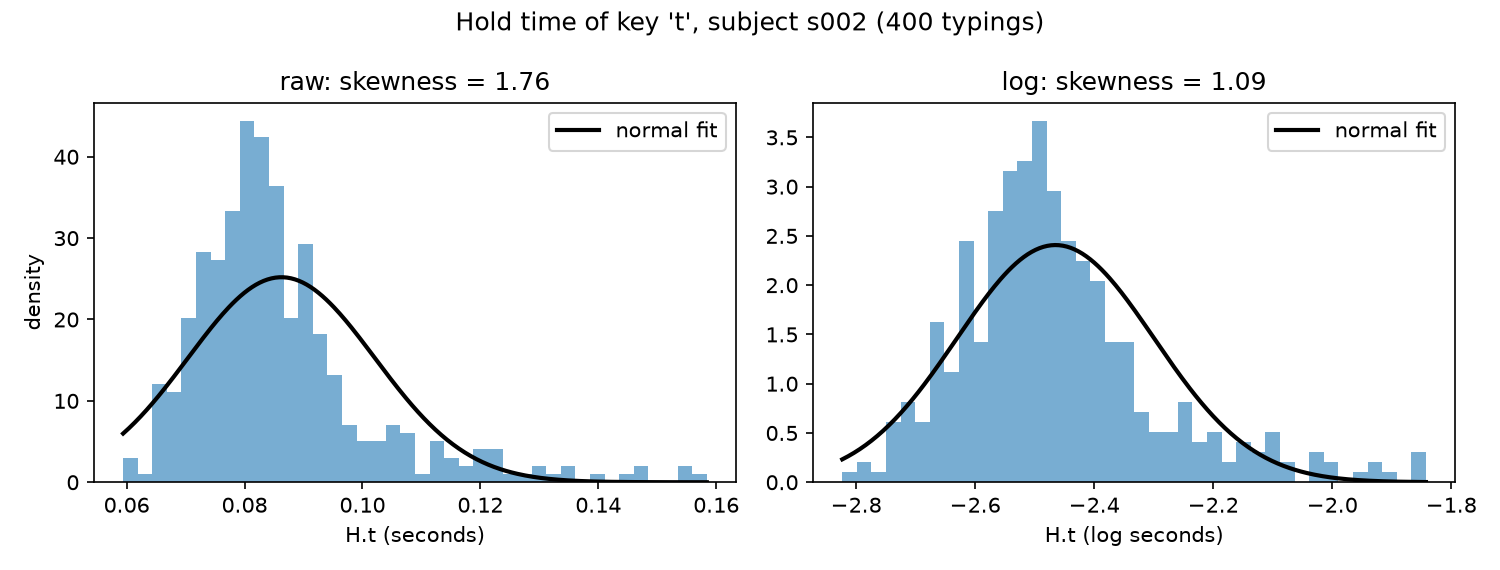
\includegraphics[width=0.95\textwidth]{real_hold_time_hist.png}
\caption{Hold time of the key \texttt{t} for subject \texttt{s002} (400 typings), raw seconds (left) and log seconds (right), with a fitted normal density. The log reduces the skewness from 1.76 to 1.09 but does not remove the right tail completely, so normality (Assumption~\ref{as:normal}) must still be checked in Iteration 3.}
\end{figure}

% Plot 2: practice / drift over sessions (Assumption 1)
\begin{figure}[H]
\centering
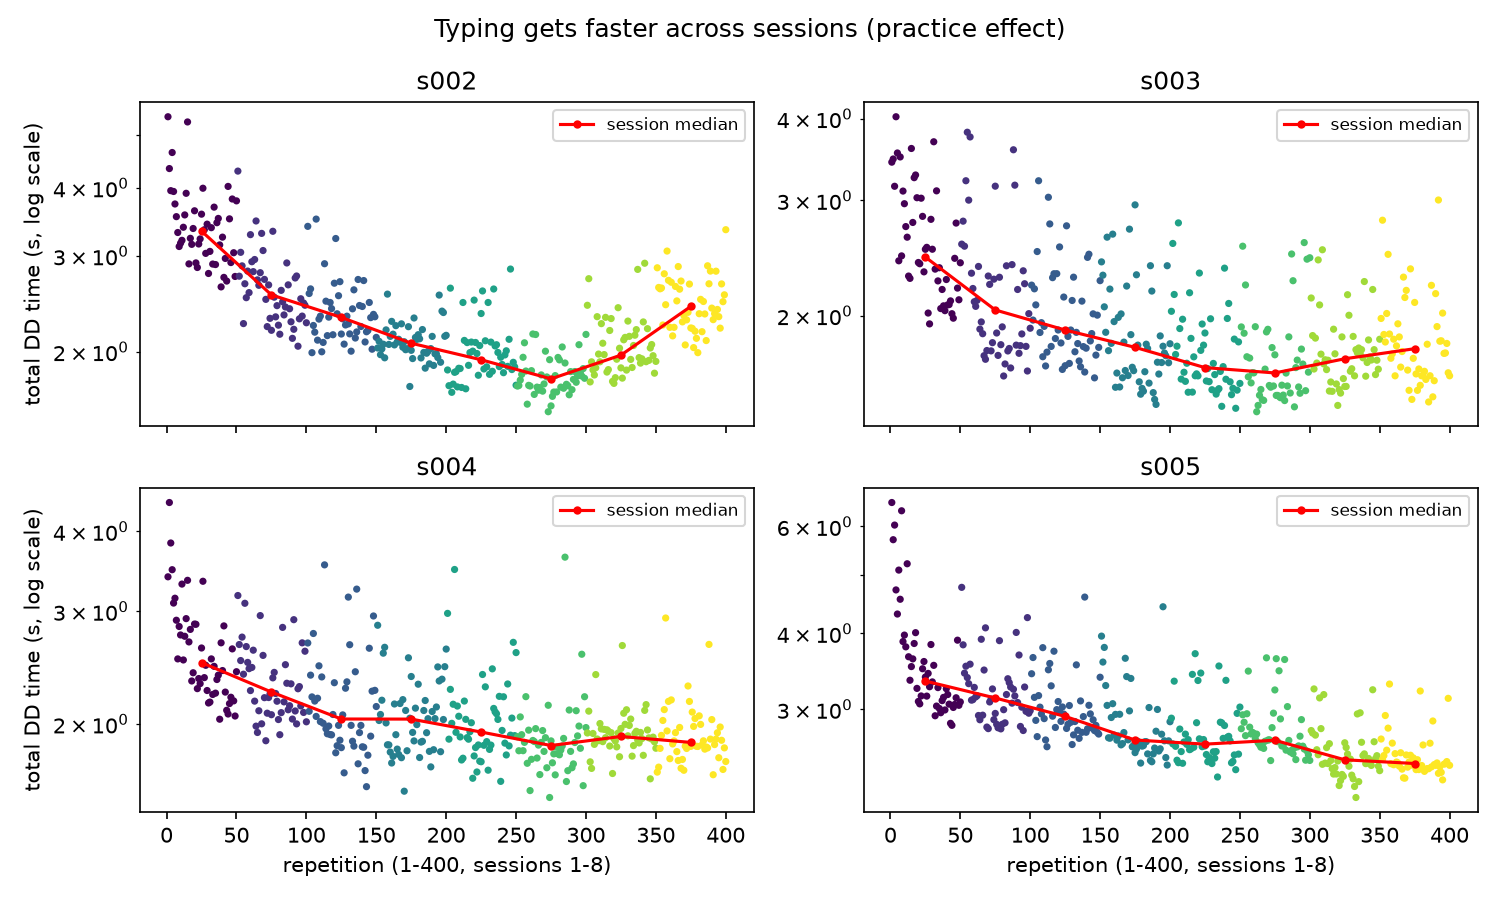
\includegraphics[width=0.95\textwidth]{real_typing_time_by_rep.png}
\caption{Total typing time (sum of the 10 \texttt{DD} latencies, log scale) against repetition $1,\dots,400$ for four subjects, coloured by session, with the session medians in red. Typing gets faster with practice: over all subjects the median total time falls from $2.71$\,s in session 1 to $1.99$\,s in session 8, with the largest drop early on. Some subjects (e.g.\ \texttt{s002}) slow down again in the last sessions. The typings are therefore not identically distributed over time (Assumption~\ref{as:iid}), and a model fitted on sessions 1--4 may raise false alarms on sessions 5--8.}
\end{figure}

\subsection{Simulation Check}
\paragraph{Model.} $\x_i \overset{\text{iid}}{\sim} \Normal(\bmu,\Sigma)$ with $d=5$, $\bmu=\mathbf{0}$, $\Sigma = BB^\top + 5I$ where $B$ has i.i.d.\ $\Normal(0,1)$ entries; $n=5000$; $\alpha=0.01$; seed \texttt{np.random.default\_rng(0)}. Code: \texttt{src/simulate.py}.

\begin{table}[H]
\centering
\begin{tabular}{@{}lrrr@{}}
\toprule
Parameter & True & Estimate & Abs.\ error \\
\midrule
$\mu_1$ & 0.0000 & 0.0529 & 0.0529 \\
$\mu_2$ & 0.0000 & 0.0013 & 0.0013 \\
$\mu_3$ & 0.0000 & 0.0228 & 0.0228 \\
$\mu_4$ & 0.0000 & 0.0089 & 0.0089 \\
$\mu_5$ & 0.0000 & $-0.0150$ & 0.0150 \\
$\Sigma_{11}$ & 5.7413 & 5.7848 & 0.0434 \\
$\Sigma_{22}$ & 9.8247 & 9.8422 & 0.0176 \\
$\Sigma_{33}$ & 12.3961 & 12.2060 & 0.1901 \\
$\Sigma_{44}$ & 7.1888 & 7.1524 & 0.0363 \\
$\Sigma_{55}$ & 8.2660 & 8.1314 & 0.1347 \\
\midrule
$\|\hSigma-\Sigma\|_F/\|\Sigma\|_F$ & --- & 0.0290 & --- \\
\bottomrule
\end{tabular}
\caption{True parameters vs.\ maximum-likelihood estimates.}
\end{table}

\begin{table}[H]
\centering
\begin{tabular}{@{}cccc@{}}
\toprule
$\alpha$ & $\tau=\chi^2_{5,1-\alpha}$ & False-alarm rate (normal) & False-alarm rate ($t_3$) \\
\midrule
0.10 & 9.2364  & 0.1010 & 0.0982 \\
0.05 & 11.0705 & 0.0516 & 0.0796 \\
0.01 & 15.0863 & 0.0102 & 0.0504 \\
\bottomrule
\end{tabular}
\caption{Observed false-alarm rates. Normal data match $\alpha$; heavy-tailed $t_3$ data do not.}
\end{table}

\begin{figure}[H]
\centering
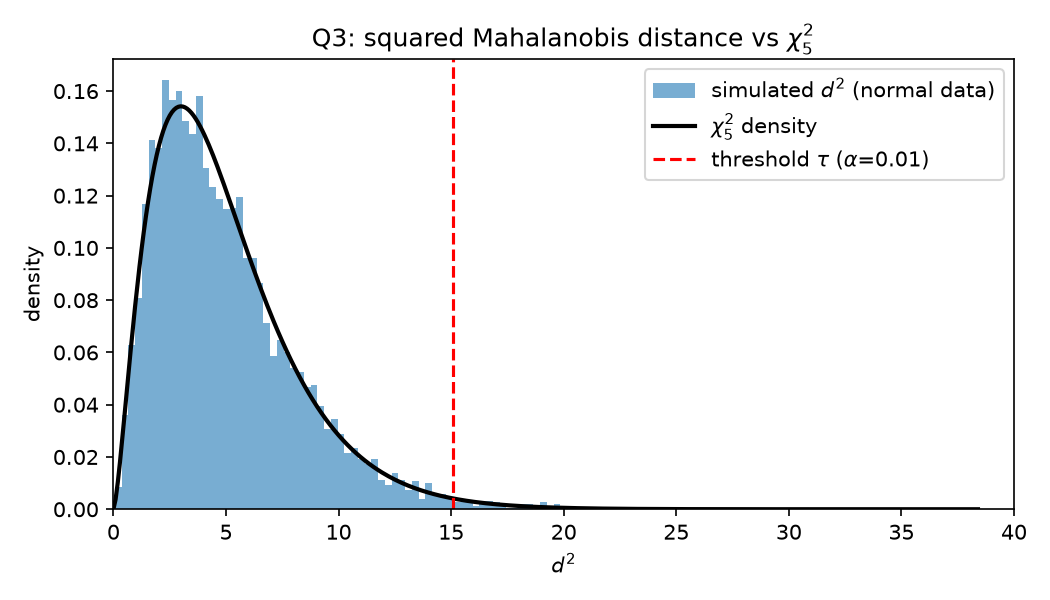
\includegraphics[width=0.75\textwidth]{sim_d2_hist.png}
\caption{Histogram of $d^2$ for the simulated normal data with the $\chi^2_5$ density and the threshold $\tau$.}
\end{figure}

\begin{figure}[H]
\centering
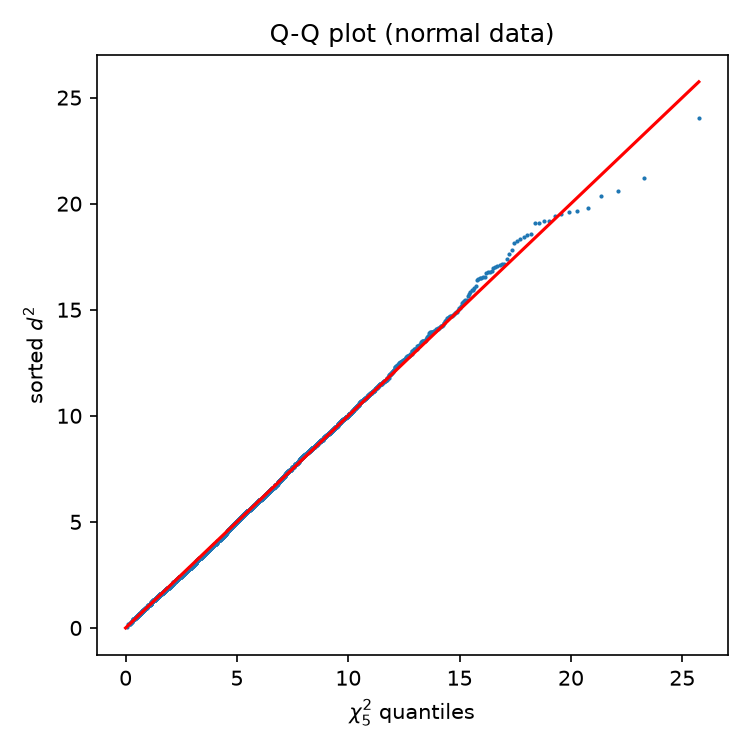
\includegraphics[width=0.48\textwidth]{sim_d2_qq.png}\hfill
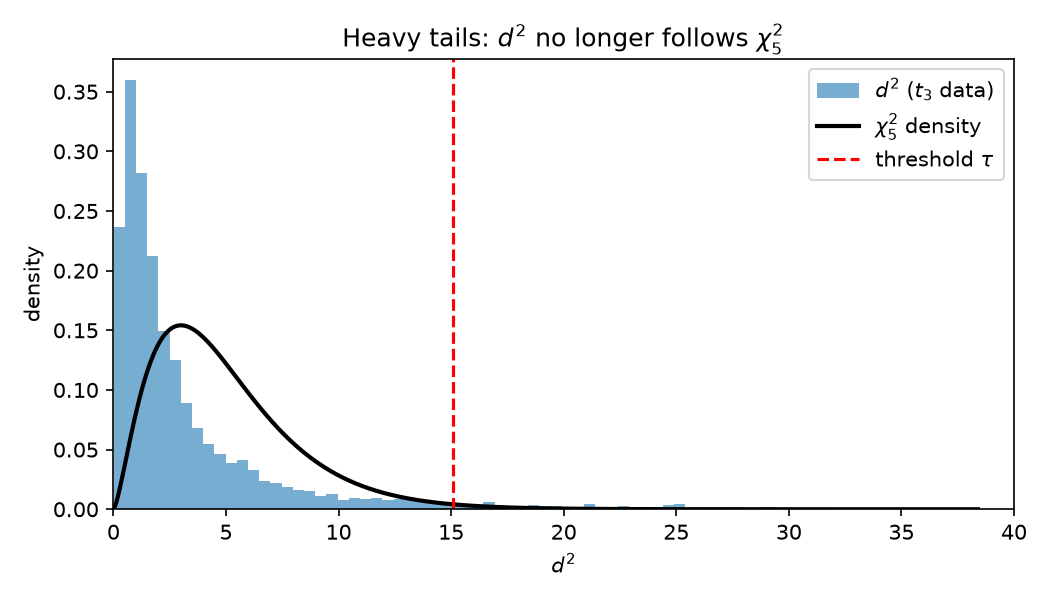
\includegraphics[width=0.48\textwidth]{sim_d2_heavy_tail.png}
\caption{Left: Q-Q plot of $d^2$ against $\chi^2_5$ (normal data). Right: $d^2$ for $t_3$ data no longer follows $\chi^2_5$.}
\end{figure}

\paragraph{What each derivation's check shows.}
\begin{itemize}[leftmargin=*]
\item \textbf{Q1:} $\hmu,\hSigma$ are close to $\bmu,\Sigma$ (relative error 2.9\%), and 20 random perturbations of $(\hmu,\hSigma)$ all lower the log-likelihood.
\item \textbf{Q2:} all eigenvalues of $\hSigma$ are positive (5.05 to 13.11) and $\min_i d^2_i = 0.060 \ge 0$.
\item \textbf{Q3:} $d^2$ has variance 10.20 (theory: 10), and a Kolmogorov--Smirnov test against $\chi^2_5$ gives $p = 0.47$.
\item \textbf{Q4:} $\hSigma^{-1/2}$ is symmetric, $\hSigma^{-1/2}\hSigma\,\hSigma^{-1/2} = I$, and the whitened data have identity covariance.
\item \textbf{Q5:} the observed false-alarm rate matches $\alpha$ at all three levels for normal data.
\item \textbf{Assumption 2:} with $t_3$ data the false-alarm rate at $\alpha = 0.01$ is 0.050, five times too high.
\end{itemize}

% ===========================================================================
\section{Member Contributions}
% ===========================================================================
\todo{One or two sentences per member.}

\end{document}
